\documentclass[conference, 11pt,slovak,a4paper,twoside]{IEEEtran}
\IEEEoverridecommandlockouts
% The preceding line is only needed to identify funding in the first footnote. If that is unneeded, please comment it out.
\usepackage{cite}
\usepackage{amsmath,amssymb,amsfonts}
\usepackage{algorithmic}
\usepackage{graphicx}
\usepackage{grffile}
\usepackage{xcolor}
\usepackage{textcomp}
\usepackage{float}
\usepackage{listings}
\usepackage[hyphens]{url}
\usepackage{pythonhighlight}
\usepackage[slovak]{babel}
\usepackage[T1]{fontenc}

\lstset{xleftmargin=2em}
\lstdefinelanguage{JavaScript}{
  keywords={typeof, new, true, false, catch, function, return, null, catch, switch, var, if, in, while, do, else, case, break},
  keywordstyle=\color{blue}\bfseries,
  ndkeywords={class, export, boolean, throw, implements, import, this},
  ndkeywordstyle=\color{darkgray}\bfseries,
  identifierstyle=\color{black},
  sensitive=false,
  comment=[l]{//},
  morecomment=[s]{/*}{*/},
  commentstyle=\color{purple}\ttfamily,
  stringstyle=\color{red}\ttfamily,
  morestring=[b]',
  morestring=[b]"
}

\lstset{
   language=JavaScript,
   backgroundcolor=\color{lightgray},
   extendedchars=true,
   basicstyle=\footnotesize\ttfamily,
   showstringspaces=false,
   showspaces=false,
   numbers=left,
   numberstyle=\footnotesize,
   numbersep=9pt,
   tabsize=2,
   breaklines=true,
   showtabs=false,
   captionpos=b
}

\lstset{
  basicstyle=\ttfamily,
  columns=fullflexible,
  frame=single,
  breaklines=true
}

\hyphenation{i-fra-me}
\hyphenation{zne-pre-hľad-ne-nia}
\hyphenation{de-tek-čnou}

\def\BibTeX{{\rm B\kern-.05em{\sc i\kern-.025em b}\kern-.08em
    T\kern-.1667em\lower.7ex\hbox{E}\kern-.125emX}}
\begin{document}

\title{Detekcia nepovoleného prístupu kustomizáciou nízko interaktívnych honeypotov}

\author{\IEEEauthorblockN{Jakub Perdek}
\textit{Slovenská technická univerzita v Bratislave}\\
Bratislava, Slovensko \\
perdek.jakub@gmail.com}

\maketitle

\begin{abstract}
Prevencia pri zabezpečení systému obvykle nemusí byť dostatočná. Z toho dôvodu je potrebné detegovať aktivity spojené hlavne s neoprávneným prístupom do systému, k súborom alebo do intranetu. Ich skoré odhalenie môže pomôcť prijať vhodné opatrenia a zabrániť reálnemu útoku na systém. Vhodným nástrojom sú práve honeypoty. Tie naviac môžu slúžiť aj na spomalenie neoprávnených aktivít alebo na zmiatnutie útočníka. Často sú ale ľahko rozpoznateľné od reálnych aktív, a preto je ich kustomizácia nevyhnutná. Lákanie možno realizovať podľa viacerých stratégií. Rovnako podľa toho možno aj prispôsobiť generovanie kustomizovateľných tokenov. Predstavujeme preto automatické riešenie pre tvorbu nízko interaktívnych honeypotov založené na čo najväčšej infiltrácii funkcionality pre sledovanie rozličných foriem manipulovania s nimi v rámci konkrétnej biznis logiky. Snahou je poskytnúť informácie o získaní konkrétnych fiktívnych informácií útočníkom. Analyzované a realizované sú preto rôzne spôsoby aplikovania uvedených mechanizmov v rámci webových dokumentov. Možnosti pre zamedzenie ich zneužitia a obmedzenie manipulácie s nimi by v rámci tohto druhu honeypotov mali byť ľahšie dosiahnuteľné a prispôsobené pre konkrétny prípad použitia.   
\end{abstract}

\begin{IEEEkeywords}
nízko interaktívne honeypoty, detekcia nepovoleného vstupu, kustomizácia honeypotov, webové honey tokeny
\end{IEEEkeywords}


\section{Úvod} \label{introduction}

Honeypoty sú bezpečnostným zdrojom, ktorý generuje upozornenie pri zachytení nadviazania interakcie s ním \cite{sanders_intrusion_2020}. Napríklad v podobe prieskumu, útoku alebo pri kompromitácii. Často lákajú infiltrovaný subjekt, a pri ich dobrom maskovaní a umiestnení môžu pomôcť odhaliť neoprávnený prístup, odhalené prístupové údaje, dokonca spomaliť aktivity útočníka vrátane odhalenia nultého útoku a rovnako aj zistiť niektoré ním pri útoku aplikované postupy. Bežní používatelia by nemali s honeypotom vôbec interagovať, ale ani vedieť o tejto funkcionalite. Prihlásenie sa do takéhoto systému alebo otvorenie a manipulácia s dokumentom, respektíve honey tokenom \cite{ng_honeypot_2018} je preto automaticky podozrivá, a malo by sa na ňu pomocou oznámení upozorniť. Honeypoty neriešia špecifický problém, a pokiaľ s nimi nikto neinteraguje ich hodnota je pre organizáciu veľmi nízka. V praxi môžu byť realizované rôznymi spôsobmi v rámci orientácie na špecifický cieľ. Tým môže byť aj detekcia neoprávnených aktivít znalých členov v organizácii vrátane možného požitia nových typov útokov \cite{spitzner_honeypots_2003}.

V našej práci sme sa zamerali na nízko interaktívne webové honey tokeny odosielajúce varovné hlásenia pri pokuse získať z nich fiktívne biznis informácie. Zamerali sme sa na možné spôsoby realizácie týchto tokenov s čo najmenšou závislosťou na ich umiestnení a procesoch nevyhnutných pre ich sledovanie, a to tak aby sme mohli zabezpečiť kustomizáciu bez závislosti na externých faktoroch.

Obsah článku je zoradený nasledovne. Sekcia~\ref{honeypotsForIntrusionDetection} charakterizuje honeypoty a ich zaradenie do kategórií s dôrazom na spôsob ich použitia. Porovnanie nízko interaktívnych honeypotov s vysoko interaktívnymi je obsahom sekcie~\ref{benefitsOfLowInteractionHoneyTokens}. Návrhom nízko interaktívnych honey tokenov je venovaná kapitola~\ref{designOfLowInteractiveHoneyToken}. Popísané sú tu možné spôsoby využitia webových technológií pri konštrukcii a následnej kustomizácii týchto tokenov. Sekcia~\ref{automatizationOfHoneyTokenCustomization} opisuje automatizáciu kustomizácie navrhnutých honey tokenov.  Návrhom a implementáciou spôsobov utajenia a zneprehľadnenia logovaného obsahu s možnosťou získania ich pôvodného obsahu aj klientskými aplikáciami sa zaoberáme v sekcii~\ref{designAndImplementationOfConcealingTools}. Sekcia~\ref{detectionLogicInsertion} približuje postup tvorby detekčnej logiky nízko interaktívnych webových honey tokenov v rámci dvoch typov. Prvý je založený na skripte, ktorý odosiela informácie na server a druhý získava dynamický obsah pomocou iframe elementu. Automatizovaným generovaním jednotlivých honey tokenov podľa predstavených spôsobov uplatňujúcich zvolenú stratégiu lákania útočníka sa zaoberá sekcia~\ref{automaticGeneratingOfHoneyTokens}. Evaluácia funkčnosti a ďalších vlastností riešenia bola vyhodnotená v sekcii~\ref{evaluationOfHoneyTokenCustomizations}. Sekcia~\ref{conclusions} sumarizuje výsledky navrhnutého spôsobu generovania a kustomizácie nízko interaktívnych honey tokenov pre detegovanie neoprávneného prístupu a predstavuje budúce možnosti smerovania práce.


\section{Honeypoty pre detekciu neoprávneného prístupu} \label{honeypotsForIntrusionDetection}

Pre detekciu neoprávneného prístupu v rámci internej siete organizácie je najvhodnejšie použiť produkčné honeypoty \cite{jahankhani_analysis_2015}. Svojou nízkou mierou false pozitív dokážu identifikovať väčšinu pokusov o vniknutie do internej siete, kompromitáciu systému alebo jeho časti. Druhou možnosťou sú aj výskumné honeypoty, ale vzhľadom na ich typické nasadenie s priamim prístupom do verejnej siete môžu byť kompromitované kýmkoľvek. Získané informácie o použitých prihlasovacích údajoch a ďalších aktivitách nie sú preto často relevantné. Zároveň by takého honeypoty mali dosahovať vyššiu mieru interaktívnosti.

Existujú rôzne techniky oklamania potencionálneho útočníka. Medzi hlavné z nich patria klamlivá služba \emph{(Deception service)}, emulácia celého operačného systému \emph{(OS emulation)}, emulácia zraniteľnosti \emph{(vulnerability emulation)}, tarpitting sieťového spojenia \emph{(connection tarpitting)}, presmerovanie spojenia \emph{(traffic redirrection)} a digitálna návnada \emph{(digital bait)} \cite{qassrawi_deception_2010}. Typickým reprezentantom pre techniku digitálnej návnady sú honey tokeny. Takýmito entitami môže byť všetko čo obsahuje falošné informácie \cite{qassrawi_deception_2010} ako napríklad fiktívny dokument alebo odkaz na neexistujúcu službu alebo produkt v konfiguračnom súbore inej služby. Manipulácia s takýmito dokumentmi má za následok vygenerovanie varovných hlásení.

Honeypot nástroje sú dostupné ako komerčné alebo aj ako open source riešenia. Príkladmi voľne šíriteľných honeypotov sú napríklad honey klient Thug a SSH honeypot Cowrie. Nízko interaktívny honeypot Thug sa používa na vyhľadanie škodlivého obsahu vrátane exploidov hlavne v javascriptovských súboroch a ďalších webových dokumentoch \cite{zulkurnain_analysis_2018}. Analýzu je možné vykonať priamo skenovaním webovej lokality alebo lokálnych súborov. Iným honey klientom je YALIH simulujúci správanie klienta na konkrétnej webovej lokalite, ktorý rovnako hľadá vzorky škodlivého kódu \cite{mansoori_yalih_2014}. Známy stredne interaktívny honeypot je Cowrie. Vďaka svojej schopnosti simulovať súborový systém umožňuje vyššiu interaktivitu s útočníkom. Tým umožňuje získať podrobnejšie informácie o útočníkových aktivitách \cite{cabral_review_2019}. K dispozícii sú preň rôzne pluginy a proxy pre protokoly SSH a Telnet. Ďalšie voľne dostupné riešenia možno nájsť v rámci pôvodných projektov na stránke honeynet.org~\footnote{\url{https://www.honeynet.org/projects/}} alebo ich zoznamy aj s popisom a odkazmi na stránkach smokescreen.io~\footnote{\url{https://www.smokescreen.io/practical-honeypots-a-list-of-open-source-deception-tools-that-detect-threats-for-free/}}\cite{smokescreen_team_open_nodate} a awesome-honeypots~\footnote{\url{https://github.com/paralax/awesome-honeypots}}.



\section{Benefity nízko interaktívnych honeypotov pre detekciu neoprávneného prístupu} \label{benefitsOfLowInteractionHoneyTokens}

Medzi úrovňou interakcie honeypotov je často potrebné robiť trade-off. Napríklad nízko úrovňové honeypoty je jednoduché nainštalovať, ľahko emulujú niektoré služby. Riziko je nízke ale rovnako je limitovaná aj poskytnutá informácia o aktivite útočníka \cite{spitzner_honeypots_2002}. Často nevyžadujú zmeny v existujúcej topológii siete alebo na zariadeniach \cite{scada_2014}. Nízko interaktívne honeypoty sú väčšinou produkčné honeypoty určené na ochranu organizácie \cite{spitzner_honeypots_2002}. Naopak vysoko interaktívne honeypoty je často náročné nainštalovať, nakonfigurovať a nasadiť. Pri použití dokerizácie je ich tvorba automatizovaná a jednoduchá aj pre nešpecializovaného administrátora. Bezpečnostný expert je potrebný aj v tomto prípade, a to kvôli monitorovaniu a analýze logov, ktoré vyžadujú znalosti slabín konkrétneho nástroja pri filtrovaní aktivít v systéme \cite{valicek_creation_2017}. Nízko interaktívne honeypoty poskytujú informácie s nízkou konkrétnosťou, a preto sa nevyžaduje ich zložitá analýza. Spravidla len upozorňujú na potencionálne nežiadúce aktivity. Pre overenie týchto aktivít sú už ale bezpečnostní experti potrební. Vysoko interaktívne honeypoty poskytujú skutočné služby namiesto simulácií, a preto pri ich zneužití predstavujú vysoké bezpečnostné riziko. Riešením pre kontajnerizované aplikácie orchestrované pomocou orchestrátora Kubernetes v prípade detegovania ich zneužitia môže byť ich automatické resetovanie \cite{reti_escape_2021}. Celkový prehľad porovnania jednotlivých typov honeypotov je vypracovaný v tabuľke uverejnenej v \cite{nagpal_catch_2015}. 



\section{Návrh nízko interaktívnych honey tokenov z webových dokumentov} \label{designOfLowInteractiveHoneyToken}

Nízko interaktívne honeypoty pre detekciu neoprávneného prístupu by mali zahŕňať mechanizmy pre generovanie informácie o príslušnej udalosti. Tie by mali byť dostatočne maskované, tak aby sa útočník o svojom odhalení najlepšie ani nedozvedel. V svojej práci sme sa zamerali na webové dokumenty. 


\subsection{Mechanizmy pre logovanie aktivity s webovým tokenom} \label{mechanismForLoggingActivity}

Analyzovali sme rôzne spôsoby vloženia spomenutého mechanizmu do webového dokumentu. Zamerali sme sa na prípady, keď sa manipuluje s webovým dokumentom neposkytovaným priamo v rámci nejakého spusteného servera. Výsledný honey token v podobe konkrétneho dokumentu bude poskytovať obmedzené možnosti interakcie s ním, a tým sa zabráni aj jeho zneužitiu. Identifikovali sme nasledovné prípady pre umožnenie sledovania interakcie s uvedeným dokumentom:

\begin{enumerate}
	\item Použitie nástroja monitorujúceho zmeny v rámci súborového systému, prípadne iného systému v rámci ktorého sa uvedené tokeny, vybrané súbory alebo dokumenty manažujú. Získaná informácia má potom podobu zistenia o identifikovanom záujme o tieto súbory. Detekčná logika využívajúca súborový systém nie je zložitá, ale v prípade jeho kompromitácie môže byť zneškodnená a rovnako je ju problematické manažovať v rámci honey tokenov samotných.
	
	\item Vloženie, respektíve nahradenie alebo upravenie existujúceho iframe elementu novým. Infiltrovanej osobe sa tým priamo poskytne hľadaný obsah aj s odoslaním informácií pri dopytoch po zdrojových súboroch nového obsahu. Zároveň možno detekčnou logikou odpozorovať o aký obsah má osoba záujem a príslušne tento obsah kustomizovať. Aj napriek tomu, ža sa iframy už neodporúča používať, tak sa stále vyskytujú napríklad pri službách poskytujúcich elektronické letáky v internetových obchodoch.

	\item Vytvorenie a odoslanie informujúcej správy, respektíve logu na server. Správu je potrebné vhodne zamaskovať, aby nebola pre útočníka čitateľná. Oproti predchádajúcemu spôsobu môže byť takáto správa odchytená, a jej odoslanie na server útočníkom znemožnené, pretože sama o sebe spravidla neposkytuje pre útočníka relevantný obsah. Preto by mala byť prepojená s vyžiadaním konkrétnych kľúčov pre sprístupnenie tohto obsahu alebo iným podmienením jeho získania útočníkom. 
\end{enumerate}
 
Obmedzenia na menované spôsoby sú zavedené z dôvodu ochrán pred internetovými hrozbami, v rámci ktorých nie je povolené zapisovať na disk pomocou prehliadača štandardným spôsobom. Rovnako ukladanie informácií alebo stavu aplikácie je obmedzené na použitie cookies, ktoré si používateľ spravidla môže prezerať. Možnosti sú preto limitované na podmienenie odoslania správy výmenou za fiktívne zdanlivo cenné informácie, ktoré sú ku dokumentu priradené.
  

\subsection{Nástroje pre maskovanie logiky honeypotu a ich význam pre kustomizáciu} \label{toolsForConcealingCustomization}

Pri tvorbe funkcionality umožňujúcej detegovať manipuláciu s týmito tokenmi a ich ďalšiu kustomizáciu sme použili nástroje pre:

\begin{enumerate}
	\item Vytvorenie kópie konkrétnej webovej lokality, prípadne len jej časti. 

	\item Manipulovanie so štruktúrou webového dokumentu a automatickú zmenu informácií v rámci nej.
	
	\item Minifikáciu a zamlženie súborov pre kaskádové štýly, skripty pre javascript a HTML dokumenty. 

	\item Využitie proxy, ktoré umožňuje získať a pozmeniť časť pravého obsahu pre nalákanie útočníka.
	
	\item Zahashovanie a zneprístupnenie obsahu až do momentu priameho vykonania skriptov na stránke. Inak by útočník mohol napríklad získať želaný obsah priamo otvorením konkrétneho súboru v textovom editore.
\end{enumerate}

Vytvorenie kópie webovej lokality sme realizovali pomocou balíčkov prístupných v jazyku Python. Pri ich reálnom použití sme zistili ich obmedzenú funkčnosť. V prípade balíčku pywebcopy~\footnote{\url{https://pypi.org/project/pywebcopy/}} to bolo časté zamrznutie skriptu kvôli zlúčeniu vlákien. Použili sme preto najnovšiu verziu priamo z githubu~\footnote{\url{https://github.com/rajatomar788/pywebcopy}} a zablokovali použitie multivláknového spracovania. Vyskytol sa ale nový problém s absolútnymi adresami skopírovaného dokumentu. Kvôli nim sa napríklad nezobrazia pôvodné obrázky na stránke. Vložili sme podporu aj pre ďalší nástroj s názvom HTTrack~\footnote{\url{https://www.httrack.com}}, ktorý je efektívnejší, a nemá uvedené komplikácie ako predchádzajúci balík. Jeho použitie je ale závislé na operačnom systéme. V súboroch necháva informácie o použití tohto nástroja, a tie by mali byť odstránené.

Príklad použitia nástroja HTTrack pre získanie súborov do hĺbky 1, bez externých závislostí, a ich uloženie do priečinku ./downloads:

\begin{lstlisting}
"C:\\Program Files\\WinHTTrack\\httrack.exe" https://www.trony.it/online/store-locator -v -r1 -\%e0 -O ./download
\end{lstlisting}


Pokiaľ je možné tak manipulujeme so štruktúru webového dokumentu dynamicky pomocou pythonovskej knižnice BeautifulSoup~\footnote{\url{https://pypi.org/project/beautifulsoup4/}}. Typickou použiadavkou je upravenie konkrétnych iframe elementov a nastavenie ich atribútov. Niekedy je potrebné funkcionalitu využiť pre prepojenie aj upravených alebo vytvorených skriptov alebo kaskádových štýlov s webovým dokumentom. Pokiaľ načítanie tejto štruktúry nie je možné, potom by malo byť zabezpečené pridanie uvedených častí v textovej podobe.

Do riešenia sme pridali niekoľko nástrojov pre zamlženie a minifikáciu súborov. Rôzne nástroje poskytovali funkcionalitu pre rozdielne formáty súborov. Pre minifikáciu HTML sme použili pythonovskú knižnicu htmlmin~\footnote{\url{https://pypi.org/project/htmlmin}} s nastavením pre vymazanie prázdneho miesta a odstránenie komentárov. Pre minimalizáciu javascriptovského kódu sme použili Closure Compiler~\footnote{\url{https://github.com/google/closure-compiler}} od Googlu. V rámci jeho konfigurácie sme nastavili compilation-level na SIMPLE\_OPTIMIZATIONS, kvôli tomu, že pri pokročilejšom nastavení dochádzalo k odstráneniu všetkého kódu pokiaľ nebol priamo exportovaný. Redundantné funkcie určené na zneprehľadnenie kódu by tak boli odstránené. Následne sme pridali parameter pre spracovanie aj javascriptovských súborov v striktnom móde. Minimalizáciu kaskádových štýlov sme zabezpečili pomocou externého nástroja Yui Compressor~\footnote{\url{https://github.com/yui/yuicompressor}} volaného podobne z príkazového riadku. Jednotlivé nástroje sme aplikovali na príslušné súbory v konkrétnej vybranej stromovej štruktúre. V praxi takýmito súbormi sú súbory klonovanej webovej lokality s implementovanou sledovacou logikou.

Ďalšiu voliteľnú časť tvorí použitie proxy pre poskytnutie časti relevantného obsahu s dodatočnou možnosťou úpravy. Funkcionalitu sme sa rozhodli pridať kvôli uľahčeniu procesu kopírovania časti namiesto celej webovej lokality, keďže v praxi táto činnosť vyžadovala kopírovanie obsahu aj z externých stránok. Reštriktívny je CORS hlavne pri zabezpečenejších aplikáciách. Namiesto proxy je preto výhodnejšie poskytovať celý fiktívny obsah pre honeypot priamo. Pri využití proxy možno reálne dáta z existujúcich služieb upravovať dynamicky počas vykonania dopytu, ale zvyšuje sa riziko odhalenia takéhoto honeypotu.

Podstatnými sú nástroje pre maskovanie obsahu. Dáta je možné uložiť do viacerých častí, ktoré sa v priebehu vykonania zložia. To núti používateľa aby súbor reálne otvoril v prehliadači, nechal vykonať kód, a tým umožnil aj vykonanie skrytej sledovacej logiky. Opäť by sprístupnenie obsahu malo podmieňovať umožnenie komunikácie so serverom, inak sledovacia logika neoznámi manipuláciu s tokenom. Rovnako je možné použiť kódovanie base64, ktorým ukryjeme obsah spolu so sledovacou logikou pred vyhľadaním zvonka. Alternatívou je prevod do hexadecimálneho formátu alebo použitie knižnice pre kompresiu a quotovanie dát. Existujú rôzne formáty, známym je napríklad gzip. 


\section{Automatizácia kustomizácie honey tokenu} \label{automatizationOfHoneyTokenCustomization}

Kustomizácia je podstatná pre zníženie pravdepodobnosti detekcie honeypotu. V praxi dochádza k fingerprintingu \cite{mohammed_honeypots_2015}, pri ktorom útočník na základe určitých charakteristických znakov odhalí honeypot. Príkladom môžu byť rôzne preklepy alebo nedostatočné schopnosti pri simulácii reálnych nástrojov. Ďalším príkladom môže byť odoslanie chybovej správy so status kódom 200 namiesto príslušného chybového kódu. Imitácia webového serveru v tomto prípade zlyhala. Pri overovaní pravosti sa útočník sústredí hlavne na tieto usvedčujúce charakteristické črty. Automatizovanie a zavádzanie náhodnosti pri kustomizácii by malo útočníkom sťažiť schopnosť takejto detekcie.

V rámci automatizácie a kustomizácie honey tokenu sme sa zamerali na dve stratégie. V rámci prvej používateľ špecifikuje počet výrazných honey tokenov a doménu z ktorej majú byť vytvorené. V rámci druhej stratégie automatizácia a kustomizácia nebude zvýrazňovať určité charakteristiky cieľového súboru a jeho obsahu ale vytvorí dostatočný počet takýchto podobných tokenov.

V rámci samotnej automatizácie sa vykonajú kroky v nasledovnej postupnosti:
\begin{enumerate}
	\item Klonovanie webových dokumentov z konkrétnej domény. Zváži sa tu aj klonovanie nepovolených stránok v rámci súboru robots.txt a hĺbka tohto klonovania.

	\item Pre každý generovaný prvok sa rovnako vykoná nasledovný postup. Vloží sa iframe element so sledovacou funkcionalitou, pri ktorom server loguje požiadavky pre dopytovanie sa po jeho obsahu alebo sa nahradí existujúci iframe aj spolu s presunutím poskytovania tohto obsahu na server. V prípade nepoužitia iframe elementu sa vygeneruje a vloží kód odosielajúci informácie pri vyžiadaní konkrétneho obsahu.
	
	\item Klonovanie webovej lokality na adrese, na ktorú odkazuje iframe element a tvorba API pre poskytnutie funkcionality vyžiadanej konkrétnym iframe elementom. Obsah v rámci biznis domény uložený v rámci konkrétnych súborov by mal byť ďalej kustomizovaný. V prípade nepoužitia iframe elementu sa vygeneruje kostra servera poskytujúceho kľúče pre sprístupnenie obsahu od klienta a odmaskovanie správy pre jej zalogovanie.
	
	\item Ďalšie zneprístupňovanie obsahu v rámci súborov. Zabezpečenie funkčnosti pri vykreslení stránky a aplikovaní kľúčov zo serveru.
	
	\item Prípadné pridanie redundantného kódu alebo spájanie a vykonanie zamlženej verzie.
	
	\item Rovnako pre každý generovaný honey token prebehne minifikácia spolu s prípadným zamlžením skriptov, html súborov a asociovaných kaskádových štýlov. 
\end{enumerate}


\section{Návrh a implementácia nástrojov pre utajenie obsahu} \label{designAndImplementationOfConcealingTools}

Ukrytie obsahu konkrétnych správ ale aj celých skriptov je v rámci statických webových dokumentov často nevyhnutné. Zároveň je potrebné aplikovať takýto postup na každú zahrnutú biznis informáciu, ktorá by neskôr mala byť sprístupnená a prezentovaná v rámci konkrétneho honey tokenu. Sprístupnia sa iba konkrétne fiktívne biznis informácie. Útočník by si potom nemal všimnúť obsah konkrétnych (logovacích) správ, ale ani správy samotné. Rovnako by nemal ani blokovať požiadavky smerujúce na server kvôli jeho potencionálnemu záujmu o biznis obsah. Uvedená funkcionalita by mala zabezpečiť doručenie rôznych druhov informácií odosielaných z rôznych častí, respektíve skriptov webového dokumentu, a zvýšiť tak možnosti informovania o činnosti útočníka.


\subsection{Utajenie obsahu kompresiou a kódovaním} \label{contentConcealing}

Pre budúci generátor honey tokenov sme navrhli funkcionalitu, ktorá bude obsah niekoľko ráz maskovať s použitím náhodne vybraných metód uplatnených zvolený počet krát. Výsledkom bude maskovaný obsah a kľúčom bude postupnosť identifikátorov metód, slúžiaci pre budúce navrátenie zamaskovaného textu do čitateľnej podoby. Funkcionalitu sme zostrojili tvorbou triedy podporujúcej dve základné metódy pre maskovanie a odmaskovanie. Konkrétne implementácie dediace od nej potom tieto metódy prekryli vlastnými využívajúcimi svoju špecifickú funkcionalitu. Umožnili tak náhradu za túto základnú triedu, čo dopomohlo k náhodnému výberu konkrétnej metódy. V základnej triede sme implementovali nástroje pre náhodný výber metódy, získanie metódy podľa identifikátora, funkcionalitu umožňujúcu maskovať a rovnako odmaskovať konkrétny obsah.

Pri implementácii konkrétnych maskovacích metód sme využili knižnice tretích strán. Okrem základnej funkcionality umožňujúcej vytvoriť z textu hash ako napríklad base64, base32, base16 alebo base85 (knižnica base64~\footnote{\url{https://docs.python.org/3/library/base64.html}}) sme implementovali aj podporu pre kompresné metódy ako je gzip (knižnica gzip~\footnote{\url{https://docs.python.org/3/library/gzip.html}}), deflate (knižnica zlib~\footnote{\url{https://docs.python.org/3/library/zlib.html}}) alebo brotli (knižnica brotli~\footnote{\url{https://pypi.org/project/Brotli}}). Vstupom ako aj výstupom každej z týchto metód je textový reťazec. Problémom kompresných metód je vrátenie výslednej hodnoty v binárnej podobe. Bolo preto potrebné zaručiť konverziu do textovej podoby. To ale v rámci kódovania utf-8 nebolo kvôli rôznym nevyhovujúcim znakom možné. Pri vynechaní chýb nebolo spätné odmaskovanie úplne úspešné a uplatnenie viacerých metód ani možné. Rovnako pretypovanie spôsobovalo chyby pri integrácii spomenutých kompresných metód. Nakoniec sa nám problém podrilo vyriešiť nástrojom pre quotovanie url (knižnica urlib~\footnote{\url{https://docs.python.org/3/library/urllib.html}}), ktorý to dokázal urobiť aj z binárnej podoby (metóda pre prevod z binárnej podoby na text má podobu urllib.parse.quote\_from\_bytes(compressed\_bytes) a metóda pre spätný prevod má podobu urllib.parse.unquote\_to\_bytes(encoded\_text)). Ako ďalšie metódy pre maskovanie textu sme použili funkcionalitu pre quotovanie url (urllib.parse.quote\_plus(pure\_text)) a jeho spätný prevod (urllib.parse.unquote\_plus(encoded\_text)).

Nakoniec sme implementovali spomenuté metódy pre maskovanie a odmaskovanie. Metóda pre maskovanie získa zo vstupu zvolený text, pole maskovacích metód a počet cyklov udávajúci koľko krát sa majú maskovacie metódy uplatniť. Následne náhodne vyberie z tohto poľa maskovaciu metódu a uplatní ju na zvolený text. Zaznamená sa aj druh tejto metódy podľa identifikátora rovnakej metódy. Postup sa opakuje zvolený počet krát vždy s predtým maskovaným textom. Výsledkom je maskovaný text a identifikátor všetkých použitých maskovacích metód ako kľúč. Ten sa môže umiestniť na serveri a zabezpečiť tak utajenie obsahu, alebo použiť na odmaskovanie obsahu už na klientovi, pričom je v tomto prípade nevyhnutné dômyselne ukryť tento kľúč. V rámci uvedenej funkcionality je predpoklad odmaskovania na klientovi dôležitý, inak by bolo vhodnejšie text rovno zašifrovať. Server by potom musel byť schopný odšifrovať konkrétne správy, respektíve informácie. Proces maskovania a odmaskovania potrebného obsahu je zobrazený na obrázku \ref{contentConcealing}.

Metóda na odmaskovanie požaduje na vstupe maskovaný text a identifikátor všetkých použitých metód pre maskovanie. V rámci tejto metódy sa vykoná reverzná aplikácia uvedených metód v opačnom poradí ako boli použité pri maskovaní. Výsledkom je odmaskovaný text v podobe v akej bol pred jeho utajením.


\begin{figure}[!t]  %vycentrovany obrazok grafu, vsadeny do odstavca
					\begin{center}
									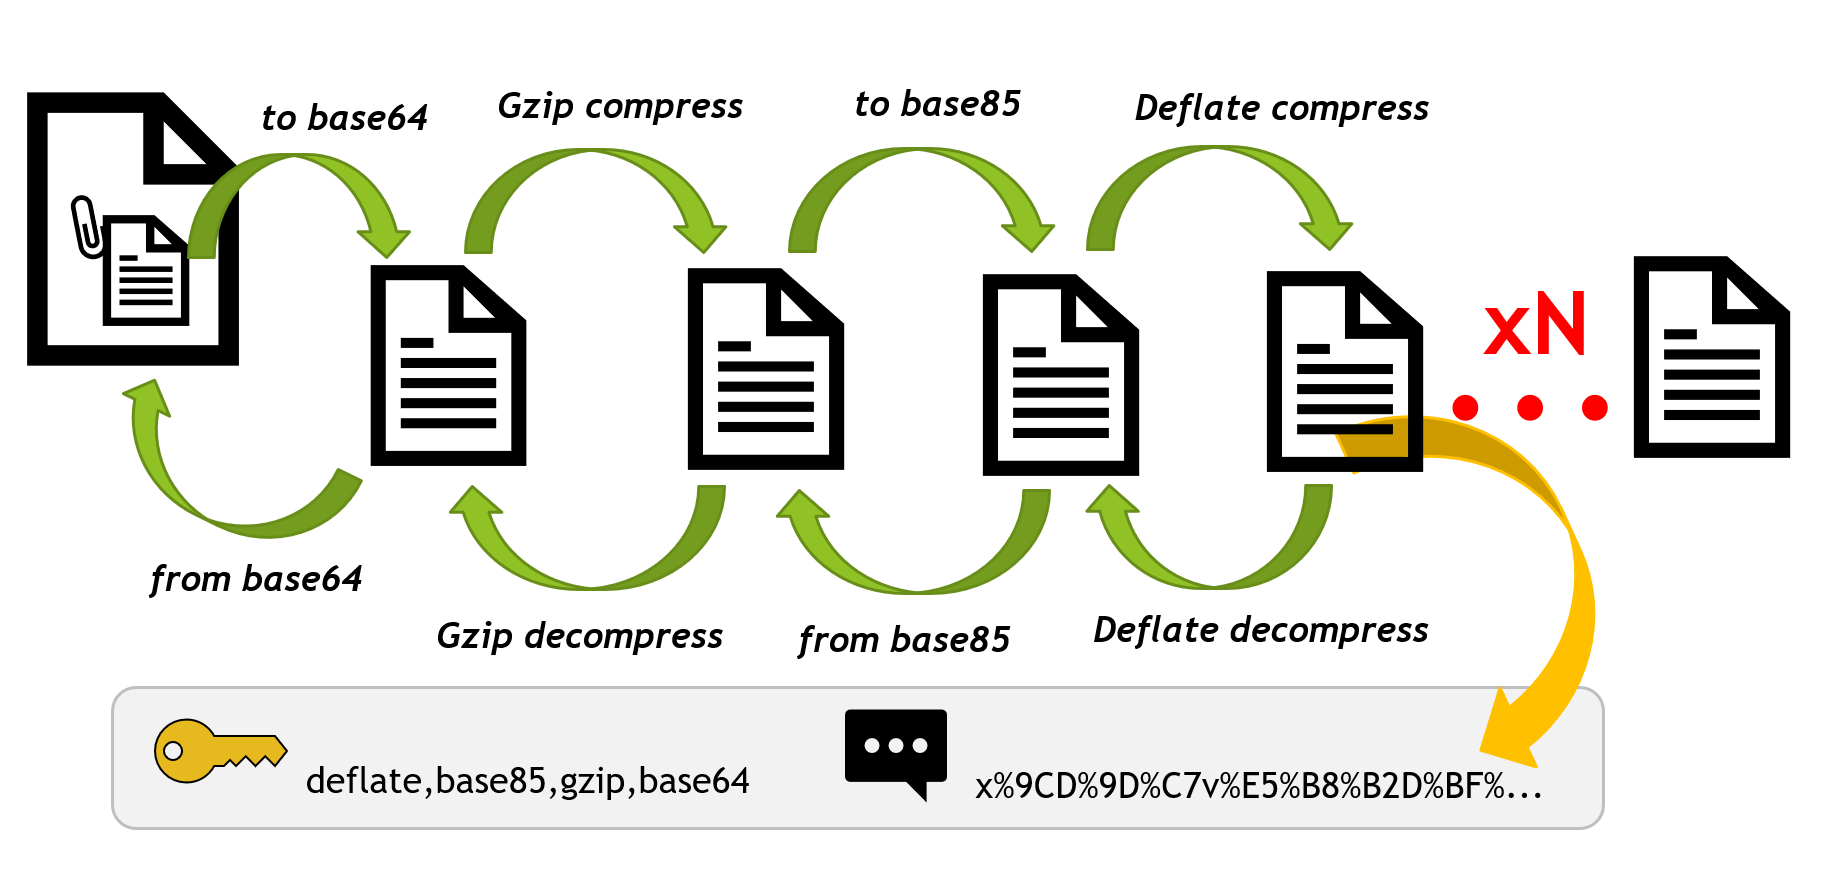
\includegraphics[width=\linewidth]{fig/masking.png}
									\caption{Maskovanie a odmaskovanie požadovaného obsahu}
									\label{contentConcealing}
					\end{center}
\end{figure}



\subsection{Zamlženie kódu jeho rozdelením a vykonaním v rámci druhého kódu} \label{codeObfuscation}

V praxi okrem štandardnej minifikácie kódu zahŕňajúcej náhradu premenných a odstránenie prázdneho miesta môže byť užitočné aj rozdelenie kódu na viaceré časti. Ak sa pred rozdelením aplikuje maskovanie obsahu z predchádzajúcej časti dostávame tak dômyselne utajený obsah. Týmto obsahom je najčastejšie správa o identifikovanej aktivite útočníka, ale môže ním byť aj samotný zdrojový kód. V prípade takéhoto spracovania zdrojového kódu ako reťazca je potrebné vykonať metódu eval. V rámci nej sa zdrojový kód zapísaný ako textový reťazec vykoná. Použitie tejto metódy je stále veľkým bezpečnostným rizikom, a preto je sa jej lepšie vyhnúť. Ideálne je predĺžiť kód jeho rozdelením na jednotlivé príkazy, lepšie prepliesť kód s bizis logikou alebo pridať nepotrebné a redundantné časta.

V rámci našej implementácie sme umožnili rozdeliť textový reťazec na viaceré časti s použitím premenných a polí. Do polí sú tieto časti pridávané priamo alebo vo forme premenných, ku ktorým boli predtým priradené. Následne je predtým rozdelený reťazec takýmto spôsobom znovu zložený. Jednotlivé príkazy sú postupne vytvárané a ukladané do poľa v poradí v akom boli vygenerované. Náhodne sa pritom aplikujú implementované metódy pre generovanie príkazov ako napríklad tvorba premennej vo forme textového poľa alebo textového reťazca a zlúčenie premenných. Dodatočne je možné pridávať medzi tieto príkazy aj iné redundantné príkazy alebo príkazy prislúchajúce ku konkrétnej biznis logike. Funkcionalitu sme testovali s aplikovaním maskovania obsahu v rámci vykonania javascriptovského kódu pomocou knižnice js2py~\footnote{\url{https://pypi.org/project/Js2Py/}}. Uvedený test možno spustiť vykonaním skriptu test\_content\_concealing.py:

\begin{lstlisting}
"./venv/Scripts/python.exe" ./content_concealing/test_content_concealing.py
\end{lstlisting}


Výstupné texty boli zhodné. Identifikovali sme aj problém s použitím deklarácií využívajúcich kľúčové slovo let, pri ktorých bolo potrebné konkrétny kód obaliť do funkcie. V opačnom prípade dochádzalo ku kolízii premenných. Použitie var namiesto let by problém vyriešilo, ale mohlo by spôsobiť aj problémy. Var by mal byť používaný len výnimočne pre globálne deklarácie. 

Príklad zamlženia kódu jeho rozptýlením do viacerých príkazov môžete vidieť na obrázku \ref{codeScattering}. V tomto prípade ale správa, ktorá je na obrázku zvýraznená modrou farbou, nie je maskovaná. Pri jej odchytení môže byť ľahko prečítaná. Url znázornené červenou farbou je rovnako čiastočne čitateľné, ale oproti samotnému obsahu správy nemôže byť pri odoslaní maskované. V prípade potreby jeho dočasného utajenia je potrebné pred odoslaním správy zabezpečiť jeho odtajnenie. Javascriptovský kód je potrebné vykonať pre zloženie jednotlivých častí do jednej. Pre tieto účely sa použije funkcia eval. Pre jednoduchosť neuvádzame prepletenie kódu s príslušnou biznis logikou.


\begin{figure}[!t]  %vycentrovany obrazok grafu, vsadeny do odstavca
					\begin{center}
									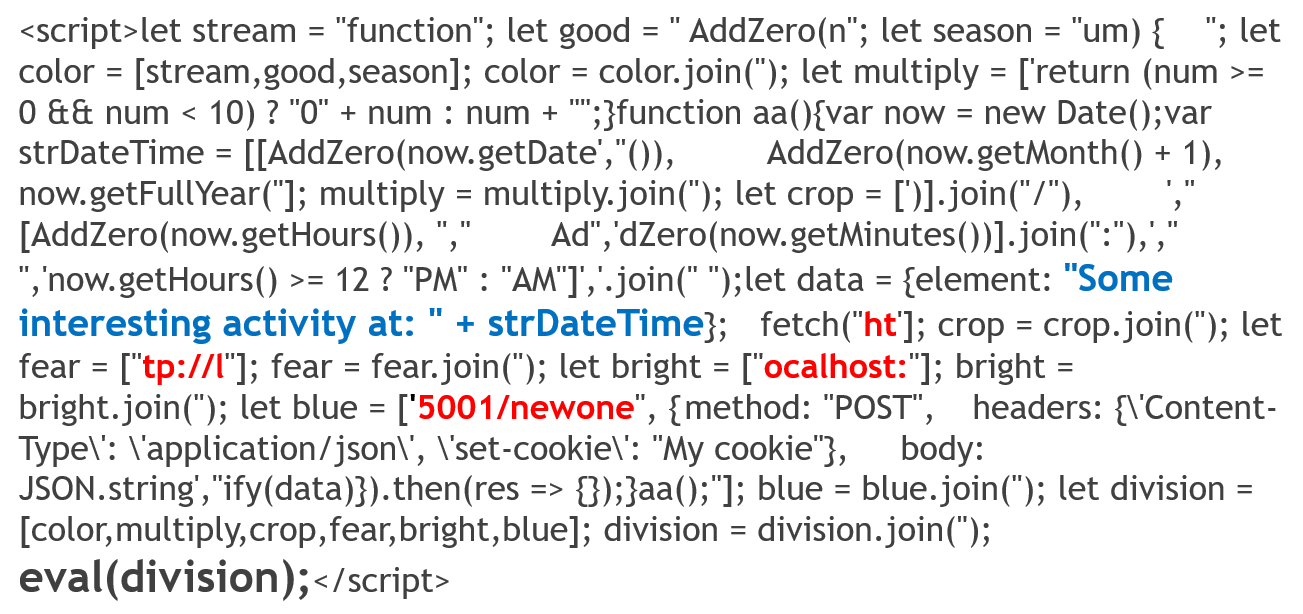
\includegraphics[width=\linewidth]{fig/codeScattering.png}
									\caption{Zneprehľadnenie kódu jeho rozptýlením}
									\label{codeScattering}
					\end{center}
\end{figure}



\section{Vloženie detekčnej logiky} \label{detectionLogicInsertion}

Detekčná logika je hlavným obsahom honey tokenu a musí byť do dokumentu vhodným spôsobom pridaná. Následne je potrebné zabezpečiť zneprístupnenie informácií a zamedziť jej odhalenie.


\subsection{Vloženie detekčného skriptu} \label{detectionScriptInsertion}

Podstatným pre využitie a prepojenie predtým realizovaných metód pre klonovanie, minimalizáciu a utajovanie obsahu je samotné vloženie detekčnej logiky v podobe správy alebo skriptu. Vzhľadom na požiadavku utajene informovať o konkrétnom obsahu by malo byť implementované aj vhodné maskovanie tejto funkcionality. Celý proces realizujeme v niekoľkých krokoch, pričom využívame náhodné generátory pre vygenerovanie rôznych parametrov určujúcich finálny výsledok:


\begin{enumerate}
	\item Príprava skriptu pre odosielanie hlásení na server. Dodatočne je možné pripraviť aj zoznam správ, ktoré sa budú posielať.

	\item Príprava webových služieb pre manažovanie logov a samotnej kostry serveru.
	
	\item Klonovanie príslušnej časti webovej lokality.
	
	\item Načítanie skriptu pre detegovanie podozrivej aktivity, prípadne aj samostatných správ. 
	
	\item Zamaskovanie buď celého skriptu, pričom v neskorších fázach bude potrebné použiť funkciu eval pre jeho vykonanie po odmaskovaní. Dôležité je maskovať obsah jednotlivých správ samostatne, aby nedošlo k úniku informácií a prezradeniu honey tokenu. Tie budú následne počas vykonávania odosielané. 
	
	\item Vloženie metód pre odmaskovanie alebo dešifrovanie konkrétneho obsahu s kódom metódy, ale nie samotných správ s dôrazom na maskovanie identifikátora použitých metód. Funkcionalita by mala byť dostupná hlavne na serveri, a to z dôvodu zistenia obsahu logov a ich následného spracovania.
	
	\item Rozdelenie obsahu do niekoľkých riadkov kódu, prípadne metód. Vhodné je aj zahrnúť tento obsah do kódu pre biznis logiku alebo pridať redundantný kód.
	
	\item V prípade zneprehľadnenia a maskovania celého skriptu je potrebné zabezpečiť odmaskovanie z neho vytvoreného kódu, a následne zavolať funkciu eval pre jeho vykonanie.
	
	\item Vloženie celého kódu do script elementu. Následne sa takto pripravený kód vloží aj do samotného honey tokenu, respektíve webového dokumentu.
	
	\item Otestovanie funkčnosti spustením serveru a otvorením honey tokenu. Odoslané hlásenia by sa mali zaznamenať.
\end{enumerate}


\begin{figure}[!t]  %vycentrovany obrazok grafu, vsadeny do odstavca
					\begin{center}
									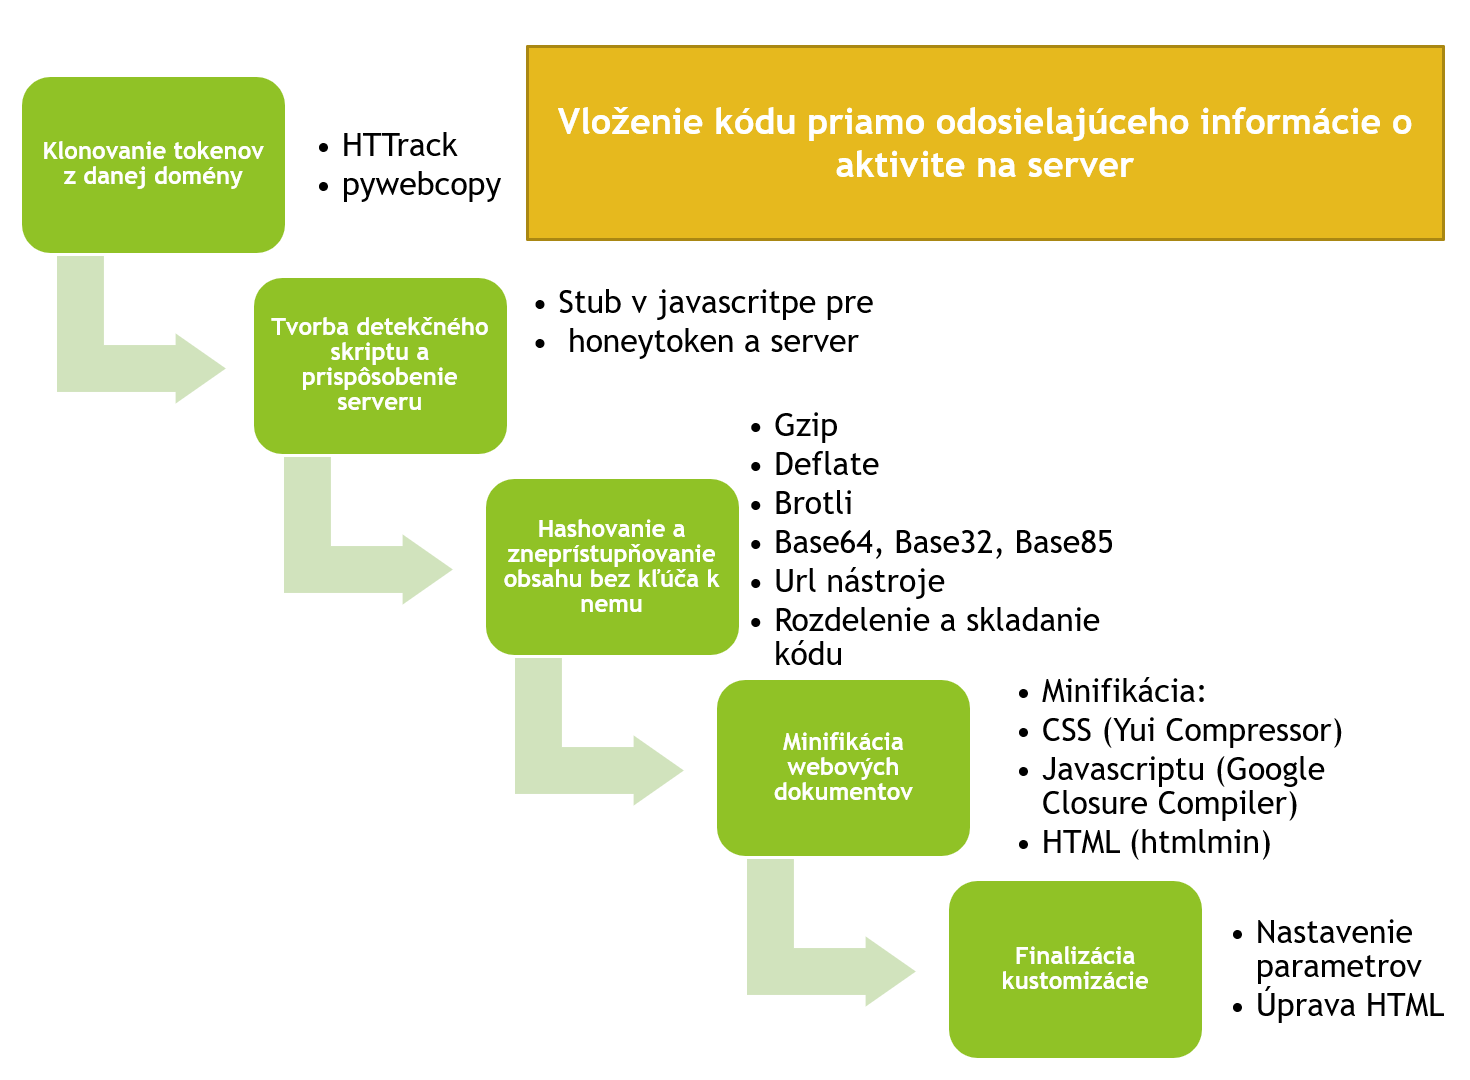
\includegraphics[width=\linewidth]{fig/senderCodeToken.png}
									\caption{Honey token s detekčnou logikou}
									\label{senderCodeToken}
					\end{center}
\end{figure}



\subsection{Injekcia iframe elementu s konkrétnym obsahom} \label{injectionOfIframeElement}

Potrebný dynamický obsah možno v rámci statického obsahu honey tokenu vložiť ako vnorený dokument pomocou iframe elementu. V konkrétnom dokumente konkrétnej webovej lokality môžeme nahradiť nejaký existujúci alebo vložiť nový. Pri nahradzovaní existujúceho by sme mali nahradiť aj celú poskytovanú biznis logiku. V niektorých prípadoch je pre tieto účely možné použiť proxi server. Druhou možnosťou je pripojiť nový iframe element, ktorý sa nemusí ani zobraziť. V tomto prípade vzrastá potencionálna šanca detegovateľnosti honeypotu. Poskytnutie reálneho obsahu tak môže byť spoľahlivejšie a zaručí to aj zabránenie blokovaniu požiadaviek na server. Aj v tomto prípade uvádzame postup tvorby takéhoto honey tokenu s dôrazom na náhodné určenie jednotlivých parametrov:

\begin{enumerate}
	\item Klonovanie príslušnej časti webovej lokality s webovým dokumentom.

	\item Vyhľadanie iframe elementu a zamenenie src atribútu za vlastnú webovú službu. Ak taký element neexistuje, alebo je komplikované napodobniť inú lokalitu, potom sa vytvorí nový iframe element s nastavenými nulovými rozmermi.
	
	\item Pokiaľ bol nahradzovaný obsah iframe elementu, potom sa zrealizuje klon webovej lokality na ktorú smeroval jeho pôvodný obsah. Následne sa tento obsah vloží do zdrojov servera pre jeho ďalšie poskytovanie honey tokenom. Inou možnosťou je prispôsobenie serveru tak, aby robil proxy medzi pôvodnou lokalitou a príslušným honey tokenom. V rámci proxy by sa niektoré informácie mali pozmeniť, aby útočník nezískal reálne biznis dáta.
	
	\item Doplnenie potrebného obsahu pre logovanie a ďalších potrebných služieb (napríklad prípadné proxy) na server.
	
	\item Maskovanie dôležitých častí obsahu vrátane biznis logiky vyššie opísanými technikami pre zmiatnutie útočníka.
	
	\item Otestovanie funkcionality spustením serveru a otvorením honey tokenu. Správa o prístupe k danému obsahu by mala byť zaznamenaná.
\end{enumerate}


Postup tvorby honey tokenu pomocou iframe elementu sme zobrazili na obrázku \ref{iframeToken}. K jednotlivým bodom uvádzame aj použité technológie.

\begin{figure}[!t]  %vycentrovany obrazok grafu, vsadeny do odstavca
					\begin{center}
									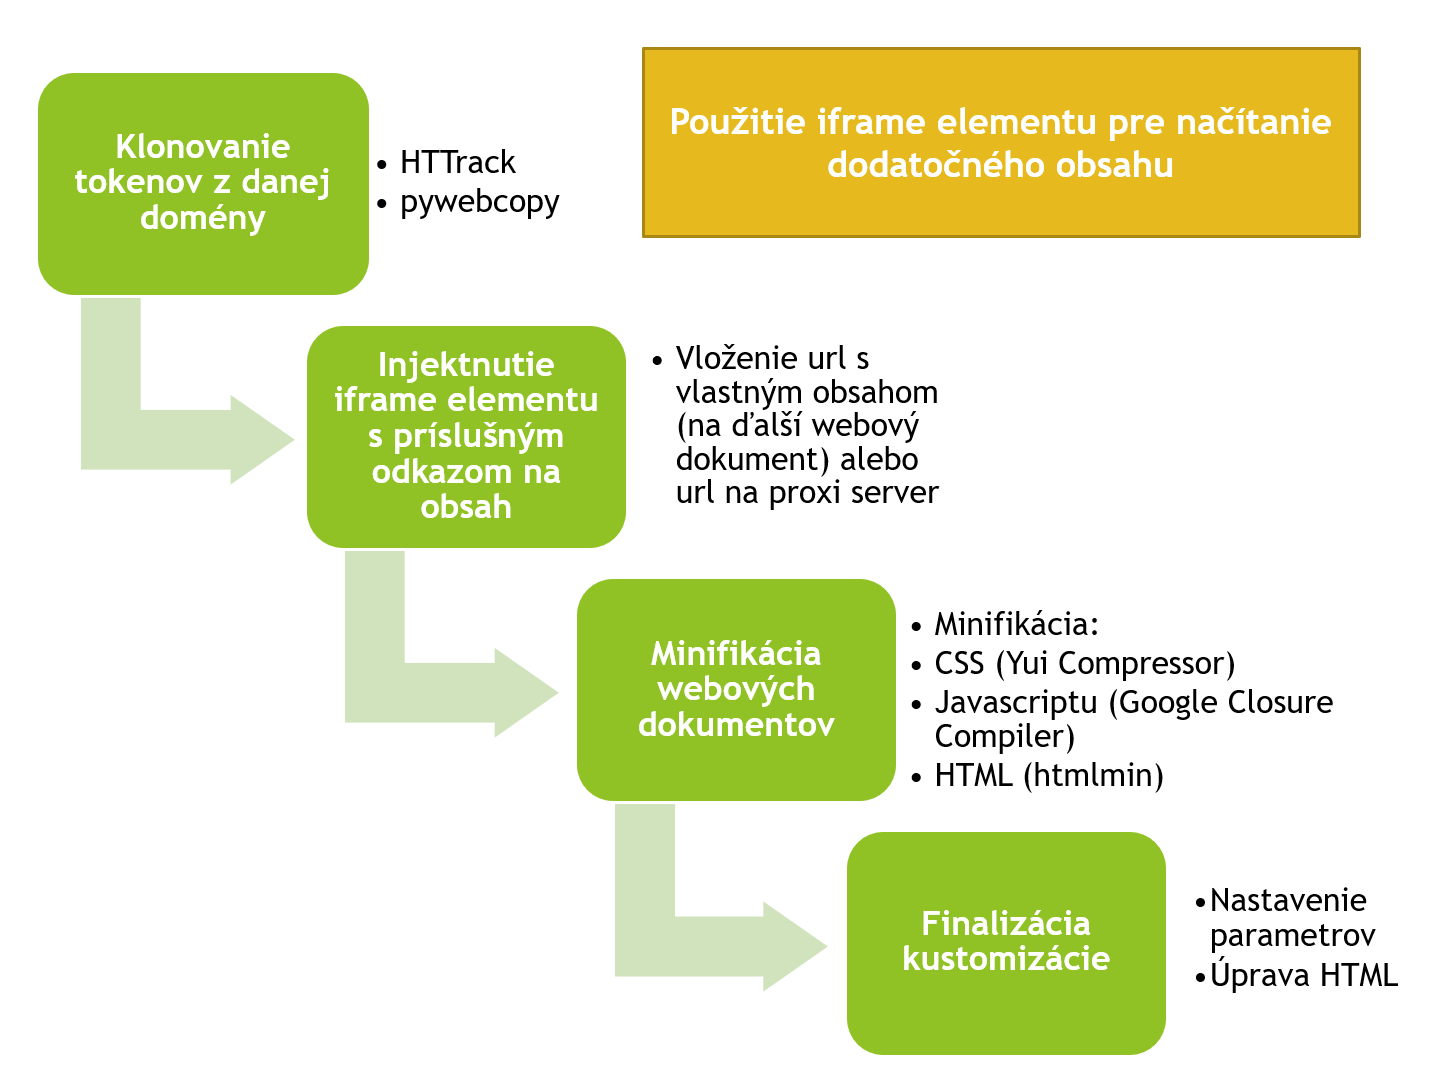
\includegraphics[width=\linewidth]{fig/iframeToken.png}
									\caption{Honey token vytvorený z iframe elementu}
									\label{iframeToken}
					\end{center}
\end{figure}



\section{Automatizované generovanie honey tokenov} \label{automaticGeneratingOfHoneyTokens}

Po návrhu kustomizovateľného honey tokenu bolo potrebné realizovať aj ich prípadné masové generovanie zosúladené so zvolenou stratégiou. Vhodné je zabezpečiť aj rozšíriteľnosť pre aplikovanie ľubovoľnej stratégie. Ich tvorbu sme preto rozdelili do niekoľkých častí. V prvej fáze sa podľa špecifických kritérií vytvorí JSON konfiguračný súbor s parametrami určujúcimi základné komponenty a ich orientáciu. Túto fázu je možné aj automatizovať. Pri automatickom vytvorení príslušného súboru, ktorému môže predchádzať získanie odkazov na podstránky konkrétnej webovej lokality, je následne potrebná manuálna revízia a úprava výsledných hodnôt konfigurácie. Druhou fázou je samotné vytvorenie konkrétnych inštancií honey tokenov a serverov podľa vytvorenej konfigurácie. Následne je vhodné manuálne upraviť výsledné časti, aby pôsobili čo najdôveryhodnejšie. Jednotlivé kroky, ktoré je vhodné aplikovať pri automatizovanom generovaní honey tokenov, sú vymenované a popísané na obrázku \ref{massHoneyTokenProduction}.

\begin{figure}[!t]  %vycentrovany obrazok grafu, vsadeny do odstavca
					\begin{center}
									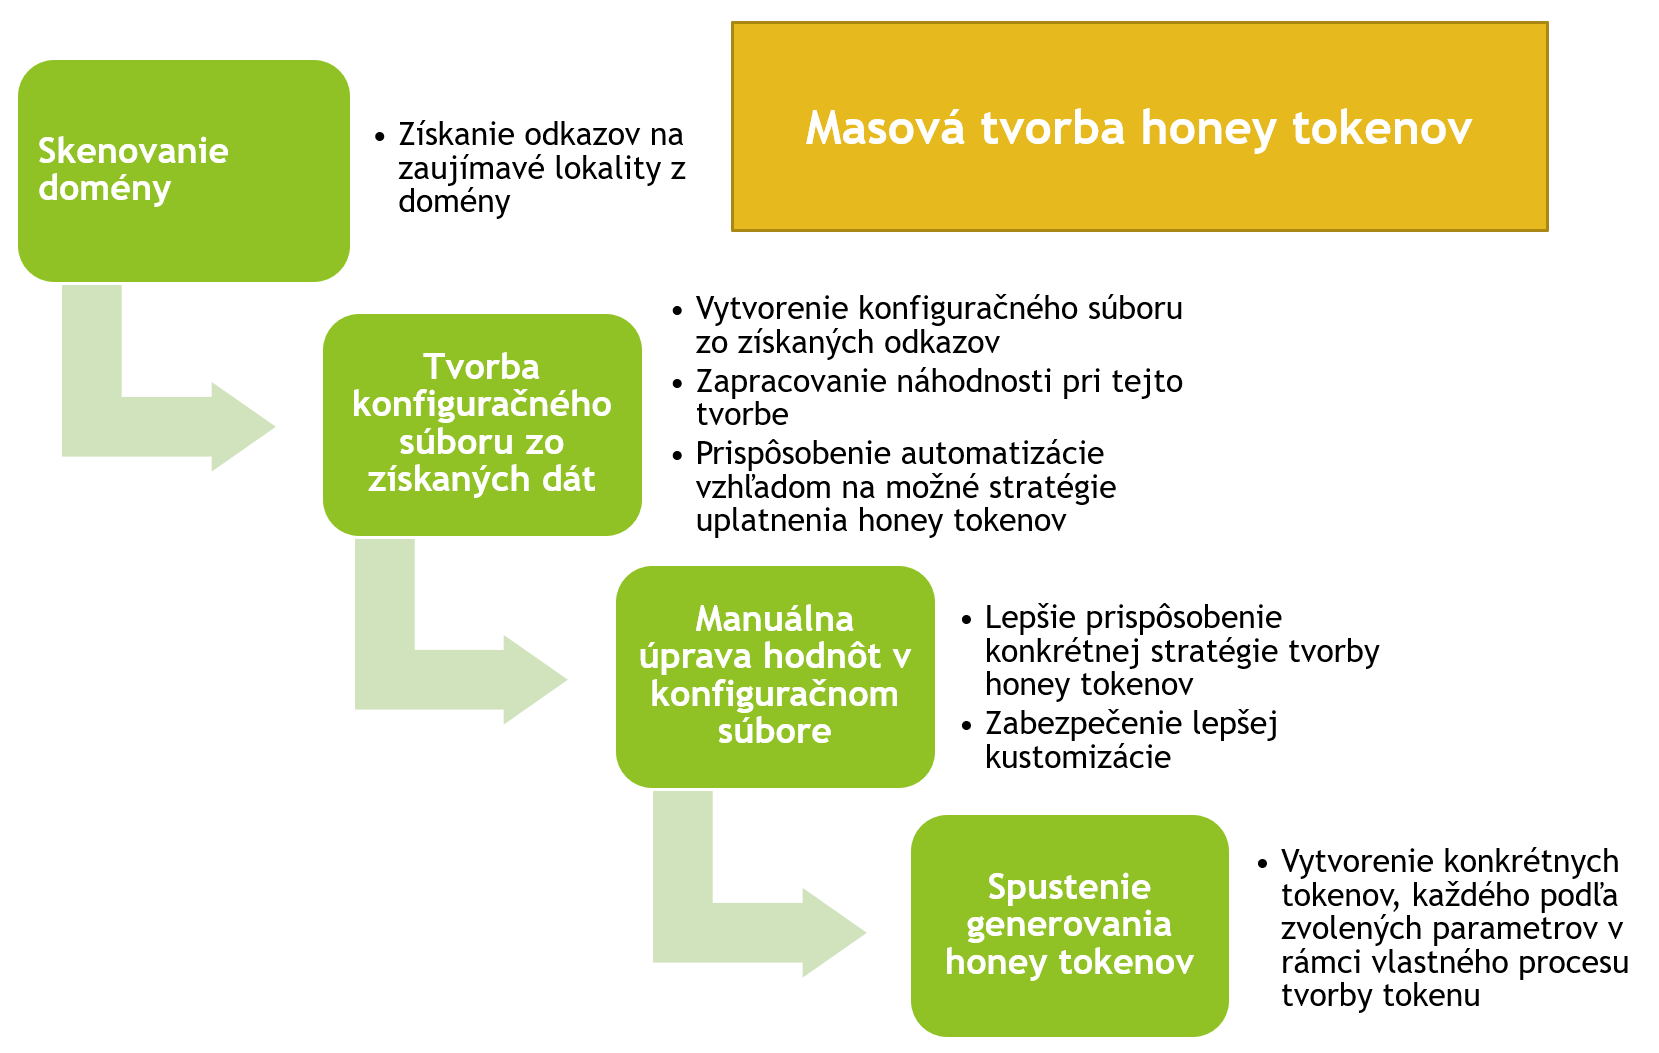
\includegraphics[width=\linewidth]{fig/massTokenGeneration.png}
									\caption{Masová tvorba honey tokenov}
									\label{massHoneyTokenProduction}
					\end{center}
\end{figure}


Zabezpečenie kustomizácie API pre komunikáciu klienta a serveru v rámci zvolenej stratégie vyžaduje určenie konkrétnych parametrov v konfigurácii pre obidve časti zároveň. Príkladom môže byť konkrétna URL na ktorej bude server získavať konrétne informácie od klienta. Server môže na tejto adrese sprístupňovať zvolený obsah, odmaskovávať skrytý obsah správ a rovnako logovať prichádzajúce správy. Klient musí byť schopný odoslať správu vo vopred navrhnutom formáte na túto URL. Pre každý honey token sa zvolí reprezentujúci odkaz na existujúci webový dokument podľa ktorého sa má vytvoriť, respektíve naklonovať. Už v tejto fáze je možné rozhodnúť o minifikácii vybraného obsahu a ďalších doplnkoch a zmenách. Okrem samotného prispôsobenia a falšovania webového dokumentu je pri konkrétnych stratégiách potrebné zvoliť aký skript sa má použiť pri komunikácii so serverom a zároveň pomocou ďalších metód aj zamaskovať. Skript by mal byť napísaný v Javascripte a obsahovať pre framework rozpoznateľné pomenovania dôležitých častí, ktoré v rámci konkretneho použitia budú dynamicky pri tvorbe honey tokenu a serveru nahradené za hodnoty z konfiguračného súboru. Príkladom takejto časti môže byť aj už spomínaná URL adresa webovej služby, ale aj reťazec identifikujúci aplikované maskovacie metódy. Podobným spôsobom sa vytvorí aj funkcionalita samotného serveru. Server môže byť vytvorený v ľubovoľnom programovacom jazyku podporujúcom nástroje pre komunikáciu s týmito dokumentami. Viacero honey tokenov by malo byť schopných komunikovať s jedným serverom. V každom z dokumentov najvyššej úrovne v konfiguračnom JSON súbore sa špecifikujú honey tokeny a práve jeden server s príslušnými rozhraniami pre ne. Vzhľadom na potrebu odovzdania informácií výhradne sieťovou komunikáciu je prítomnosť serveru nevyhnutná. Ukážka konfigurácie vybraného dokumentu nachádajúceho sa v zozname príslušných dokumentov umiestnenom v konfiguračnom súbore je zobrazená na obrázku \ref{configurationFile}.

\begin{figure}[!t]  %vycentrovany obrazok grafu, vsadeny do odstavca
					\begin{center}
									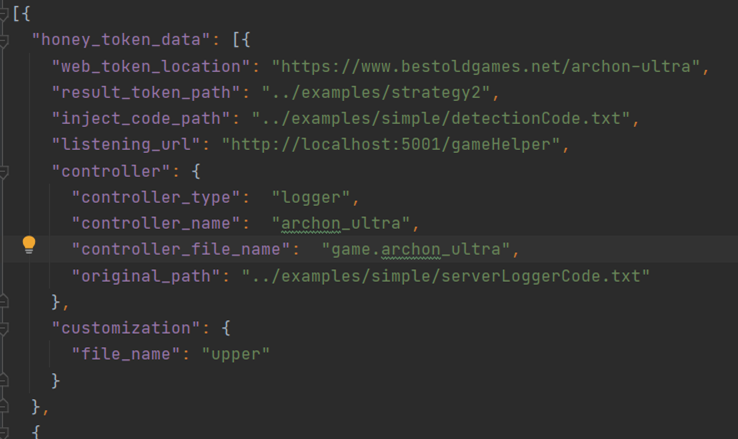
\includegraphics[width=\linewidth]{fig/configurationFile.png}
									\caption{Ukážka časti konfiguračného súboru}
									\label{configurationFile}
					\end{center}
\end{figure}



Nami vytvorené riešenie podporuje automatické generovanie častí NodeJS~\footnote{\url{https://nodejs.org/en/}} serveru. V jednoduchom prototype sa skopíruje nevyhnutná funkcionalita a postupne sa pridávajú ďalšie časti, ktoré sa podľa potreby upravujú podľa hodnôt v konfiguračnom súbore. Samotné metódy pre spracovanie príchodzích dopytov by mali byť rovnako napísané v oddelenom súbore s rozpoznateľnými hodnotami pre používaný rámec. Kód z týchto súborov rámec podľa konfigurácie zahrnie na príslušné miesto. Pri realizácii konkrétnej stratégie je tak potrebné napísať niekoľko takýchto súborov s príslušnou funkcionalitou. 

Vhodná konfigurácia môže pomôcť hlavne pri tvorbe výrazných honey tokenov lákajúcich svojím vzhľadom. Môže to byť napríklad dodatočné generovanie odkazov na konkrétny token alebo napísanie názvu súboru veľkými písmenami. Prevažná väčšina ostatných súborov by potom už nemala mať podobné prvky a pôsobiť tak pre útočníka nezaujímavo. Iná stratégia založená na podobnosti väčšiny zo súborov je obvykle priamo podporená pri tvorbe konfiguračného súboru, keďže existujúce dokumenty obvykle možno rýchlo získať priamo z webovej domény, a zároveň pre ne netreba uplatniť kustomizáciu vo vyššej miere oproti predchádzajúcej stratégii. Obsah týchto dokumentov by ale mal byť fiktívny, aby dokumenty nemohli byť ďalej zneužité.

V rámci testovania automatickej tvorby honey tokenov sme napísali krátke konfiguračné súbory pre obidve stratégie. Generátor tak vytvoril 3 tokeny, pričom sa pre každý uplatnil osobitný postup jeho tvorby. Postup je opísaný v predchádzajúcich kapitolách. Zároveň sa pre zadefinovanú skupinu vytvoril server s možnosťou prímať a spracovať dopyty od týchto tokenov. Vytvorenému serveru sme doinštalovali potrebné balíčky a spustili ho. Následne sme otvárali jednotlive honey tokeny v prehliadači. V konzole serveru následne po každom otvorení takéhoto súboru pribudol jeden záznam. Po otvorení súborov bol obsah skriptov roztrieštený v kóde pričom naň boli aplikované niektoré maskovacie metódy. Tokeny vyzerali rovnako ako pôvodné webové dokumenty. Príklad tvorby honey tokenov na základe pripravenej konfigurácie pre dve základné stratégie možno spustiť vykonaním skriptu honey\_token\_generator/honey\_token\_strategies\_generate.py. 

Po vygenerovaní príslušných častí je potrebné ešte doinštalovať potrebné balíčky pre spustenie servera a prípadne vytvorené tokeny vhodne umiestniť. Samotné umiestnenie tokenov a servera je možné nastaviť aj v konfiguračnom súbore. V prípade NodeJS servera je pre inštaláciu možné použiť príkaz 

\begin{lstlisting}
npm install
\end{lstlisting} 

a pre jeho spustenie 

\begin{lstlisting}
npm start
\end{lstlisting}.  



\section{Evaluácia tvorby a kustomizácie honey tokenov} \label{evaluationOfHoneyTokenCustomizations}

Funkčnosť a schopnosť utajiť konkrétny obsah pred útočníkom v rámci navrhnutého postupu zo subsekcie \ref{detectionScriptInsertion} sme sa rozhodli overiť automatizáciou tvorby spomenutého honey tokenu a otestovať rôzne podoby manipulácie s ním. Automatizované riešenie tvorby honey tokenov vyžaduje špecifikovanie príslušných parametrov vrátane skriptu umiestneného v samotnom honey tokene a kódu časti ovládača umiestneného na serveri. Honey token by mal byť schopný odoslať utajenú správu na server a vyžiadať si potrebný obsah. To by malo byť zabezpečené jednoduchým dopytom. Dôležité je sa zamerať na ukrytie tejto funkcionality aplikovaním vhodných metód popisovaných v predchádzajúcich častiach. V rámci automatizácie toto maskovanie realizujeme až pri samotnom vytváraní honey tokenu, a preto nie je v samotnom pripravenom kóde (\ref{maskingClientCode}) prítomné. Zároveň takéto spracovanie umožňuje použiť akýkoľvek skript.


\begin{lstlisting}[float=t,language=JavaScript,numbers=left,caption={Detekčný skript - klientská časť.},label=maskingClientCode]
function AddZero(num) {
    return (num >= 0 && num < 10) ? "0" + num : num + "";
}
function aa(){

let data = {element: <<[data]>>};
   
fetch("http://localhost:5001/input", {
	method: "POST",
	headers: {'Content-Type': 'application/json', 'set-cookie': "My cookie"}, 
	body: JSON.stringify(data)
}).then(res => {
});
}
aa();
\end{lstlisting}


Funkcionlita na serveri by mala byť schopná príslušnú správu odmaskovať a zalogovať. Zdrojový kód implementovaného riešenia pre NodeJS vykonávajúci tieto úlohy je uvedený vo výpise kódu \ref{maskingServerCode}. Využívame tu knižnicu python-shell pre vykonanie pythonovského skriptu. Po získaní odpovede z post dopytu na príslušnom url prenášanej v rámci objektu req je potrebné dekódovať jej obsah z base64 kódovania, ktoré bolo nevyhnutné aplikovať kvôli rozdeleniu príslušného kódu do skriptu. Pokiaľ by sa nevykonalo nemusel by byť príslušný skript v rámci honey tokenu platný kvôli zamiešaniu znakov z HTML formátu a problémom s quotovaním. V rámci objektu options sa nastavia parametre pre vykonanie skriptu ako sú napríklad jeho argumenty. Následne sa vytvorí objekt PythonShell obsahujúci názov príslušného skriptu spolu s konfiguráciou, ktorá bola predpripravená v predchádzajúcom kroku. Pomocou volania funkcie send pošleme skriptu zamaskované dáta zo vstupu. Rovnako je potrebné registrovať poslucháča na udalosti s názvom 'message', ktorý umožňuje logovať akýkoľvek výstup zo skriptu. Týmto výstupom v našom prípade bude odmaskovaná správa. Takýmto spôsobom možno spracovať aj dáta s väčšou veľkosťou. Ukončenie práce so skriptom je realizujované pomocou funkcie end. V rámci nej môžeme zalogovať prípadné vzniknuté chyby spojené s vykonaním skriptu.

\begin{lstlisting}[float=t,language=JavaScript,numbers=left,caption={Logovanie obsahu - serverovská časť},label=maskingServerCode]
const PythonShell = require('python-shell').PythonShell;
router.post('/replaceMe', function(req, res){
   	var concealedData = req.body.element;
	let buff = Buffer.from(concealedData, 'base64');
	concealedData = buff.toString('ascii');

	let options = {
 		mode: 'text',
  		pythonOptions: ['-u'], // get print results in real-time
  		args: ['-unconcealing', '-key', '<<[key]>>']
	};
	var pythonShell = new PythonShell('content_concealing_script.py', options);
	pythonShell.send(concealedData);

	pythonShell.on('message', function (message) {
  		console.log("FINAL LOG:");
  		console.log(message);
	});

	// end the input stream and allow the process to exit
	pythonShell.end(function (err,code,signal) {
  		if (err) console.log(err);
	});
	
});
\end{lstlisting}


Po vygenerovaní celého riešenia ručiaceho za vykonateľnosť predchádzajúcich nevyhnutných kódov sme funkčnosť funkcionality aj otestovali. Nainštalovali sme vhodné balíčky pre NodeJs server a zabezpečili podporu pre Python spolu s knižnicou brotli~\footnote{\url{https://pypi.org/project/Brotli/}}. Následne sme spustili vytvorený NodeJS server. Honey token sme staticky skontrolovali prečítaním jeho obsahu. Asociované súbory boli minifikované a skript v nich zneprehľadnený. Správa informujúca o podozrivej aktivite bola príslušne zamaskovaná. Na záver sme spustili program BurpSuite~\footnote{\url{https://portswigger.net/burp}} a otvorili v ňom honey token. V rámci rôznych dopytov sme odchytili aj dopyt s obsahom tejto správy. Obrázok \ref{burpSuiteCapturing} zobrazuje túto zachytenú správu zobrazenú programom BurpSuite. V tejto implementácii sme správu vhodne zamaskovali, preto mal útočník znemožnené vidieť jej obsah. Stále môže túto správu zahodiť, a zabrániť tak jej odoslaniu. Povolenie odoslania tejto správy by preto malo byť podmienené výmenou za fiktívny obsah z konkrétnej domény. 

\begin{figure}[!t]  %vycentrovany obrazok grafu, vsadeny do odstavca
					\begin{center}
									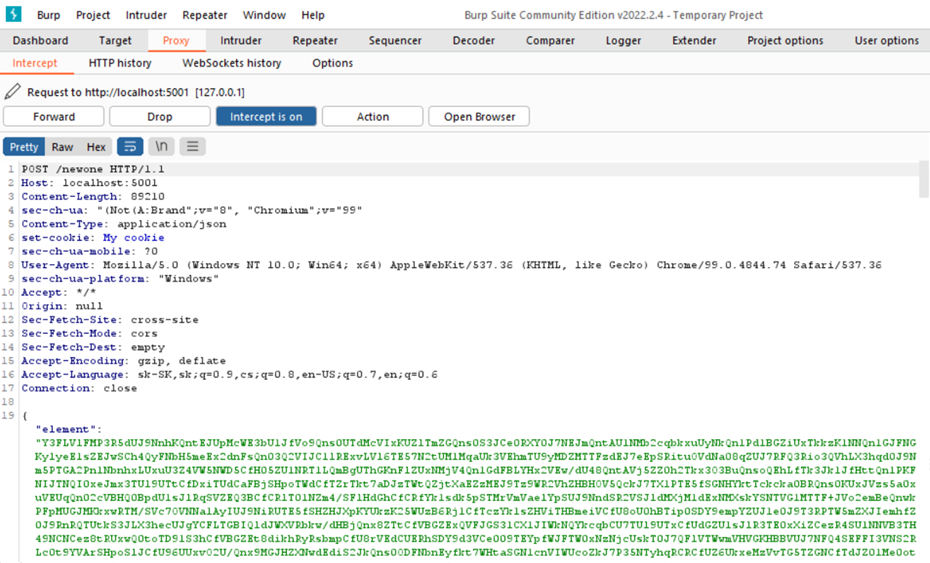
\includegraphics[width=\linewidth]{fig/burpSuite.png}
									\caption{Odchytenie výstražnej správy}
									\label{burpSuiteCapturing}
					\end{center}
\end{figure}

Uvedený príklad možno otestovať vykonaním skriptu honey\_token\_generator/honey\_token\_constructor.py a uskutočnením popisovaných krokov. Po zapnutí serveru a znovu vygenerovaní tokenu je potrebné server opäť kvôli zmene kľuča reštartovať. Zdrojový kód opisovaného riešenia je uložený v rámci github repozitára~\footnote{\url{https://github.com/jperdek/tokenCreator}} a rovnako je aj k dispozícii pre ďalšie vylepšenia.



\section{Zhrnutie a budúca práca} \label{conclusions}

Kustomizácia je pri honeypotoch veľmi dôležitá hlavne kvôli zmenšeniu miery ich detegovateľnosti. Zautomatizovanie procesu ich tvorby spolu so zavedením náhodného výberu spomedzi možných vlastností pomáha urýchliť ich vývoj a znížiť aj úsilie potrebné pre spomenutú kustomizáciu. Navrhli a vytvorili sme preto program umožňujúci nielen vytvoriť a do istej miery aj prispôsobiť konkrétne honey tokeny, ale uplatniť celý proces v rámci konkrétnej stratégie lákania útočníka. Rozmiestnenie ako aj nasadenie týchto honey tokenov realizujeme niekoľkými spôsobmi. Pri niektorých sa predpokladá vytvorenie veľkého množstva podobných inštancií, pri inom len nízky počet tých výrazných. Okrem samotných webových dokumentov sa vygeneruje jeden alebo viac serverov a služby zabezpečujúce logovanie správ z honey tokenov. Riešenie sme obohatili o techniky ukrytia obsahu, logovania správ a stiahnutia predlôh tokenov z konkrétnej webovej lokality pre ich ďalšiu kustomizáciu. Implementácia bola realizovaná podľa požiadaviek pre zabezpečenie detegovania aktivity motivovanej záujmom útočníka o konkrétne informácie špecifického webového dokumentu..

Celkovo sme vytvorili dva zakladné typy honey tokenov. Jeden využíva iframe elementy a druhý obsahuje funkcionalitu umožňujúcu odosielať správy. Funkcionalita fungujúca ako proxy, ktorá zároveň pozmeňuje prebratý obsah nie je niekedy funkčná a použiteľná z dôvodu blokovania CORS politikou. Kustomizácia je preto pracnejšia. Ďalšou zistenou nevýhodou je, že iframe elementy sú zastaralé, a často aj podozrivé pokiaľ priamo neprispievajú svojím obsahom na stránke. Obvykle vtedy majú nastavený rozmer na nulové hodnoty. Stále sa však vo veľkom počte aplikácií používajú na sprístupnenie vloženého obsahu akým sú napríklad elektronické letáky pri eshopoch. Zabezpečili sme preto klonovanie upravených informácií, ktoré budú dynamicky pomocou iframe elementu do dokumentu pri jeho otvorení vložené. Druhý typ používa skript pre odosielanie správ. Ten vyžaduje dômyselnejšie utajenie obsahu správy a zamedzenie jej blokovania pri možnom odchytení. Riešenie sme preto obohatili nástrojmi pre minifikáciu webových dokumentov a ich častí, rezdelením kódu na menšie časti a prepletením s biznis logikou, ale aj zapracovaním postupného generovania obsahu až po otvorení dokumentu v prehliadači.

Tvorbu honey tokenov sme parametrizovali a umožnili ich realizáciu podľa konfiguračného súboru. Tieto súbory obsahujú aj parametre jednotlivých webových serverov. Ich tvorba môže byť tiež automatizovaná získavaním odkazov na konkrétne časti webovej lokality akými môžu byť konkrétne produkty spolu s následnou kustomizáciou. Hlavným cieľom je doladenie niektorých kustomizačných parametrov pri uplatnení navrhnutej stratégie lákania útočníka v rámci jeho potencionálneho záujmu o konkrétne webové dokumenty pre určitú biznis doménu. Samotná realizácia dvoch základných stratégií potvrdila možnosť rýchleho vytvorenia vysokého počtu funkčných honey tokenov prispôsobených nielen svojím obsahom ale aj ladiacich dokopy ako jeden celok imitujúci potencionálny cieľ v rámci špecifickej domény. Celý proces aj v závislosti od domény vyžaduje pre čo najvyššie zvýšenie dôveryhodnosti celého riešenia vhodnú modifikáciu klonovaných informácií z konkrétnej domény ako aj dodatočnú kustomizáciu vygenerovaného riešenia. Kľúčovým pri tvorbe honey tokenov je identifikovanie útočníkovho záujmu o konkrétne informácie z domény a ich následné zahrnutie do vytvoreného riešenia.

V ďalšej práci by sme chceli pridať viac parametrov pre konfiguráciu webových honey tokenov. Rovnako by sme chceli vhodným spôsobom zabezpečiť čo najednoduchšie použitie proxi v rámci iframe elementov bez zásahov do pôvodnej biznis funkcionality. Vhodným by bolo zabezpečiť aj automatickú tvorbu konfiguračného súboru pre konkrétnu doménu spolu s prispôsobením pre aplikovanie špecifickej stratégie.

\bibliographystyle{abbrv} % plain or alpha are fine, too
\bibliography{honeypots}


\end{document}
